\section{Proofs of Construction}\label{sec:reasoning}

- approach to proving the correctness of our state channel network protocol

- the nature of state channels tends to make the logic complex
- value is moved between participants by exchanging statements about the distribution of assets held on-chain
- inevitably you end up reasoning about the statements you hold and their interpretation by the chain, and the possible actions of the other participants in the channel

- inherent danger, funds are locked on-chain
- participants act maliciously and stop cooperating at any point in the protocol
- safe at all times

\subsection{Channel Funding and Value}

We will start by considering the interpretation of the outcome of a state channel.
Suppose $A$ is a participant in a state channel, $L$, that reaches an (allocation) outcome, $\omega$, that allocates $x$ coins to $A$.
What does that mean for $A$?
In particular, how much more can $A$ withdraw from the system due to that outcome?
Understanding this is key to analysing state channel networks.

\begin{figure}[h]\centering
  \makebox[\textwidth][c]{\begin{tikzpicture}[node distance=0.3cm]
  \node (outcome) at (0, 0) {
    \begin{tikzpicture}[x=0.7cm]
      \node[circAB, label=right:$L$] (L) at (0, 0) {};
      \node[circA, label=below:$A$] (A) at (-1, -1) {};
      \node[circB, label=below:$B$] (B) at (1, -1) {};
      \draw[->] (L) edge node[midway, left] { $3$ } (A);
      \draw[->] (L) edge node[midway, right] { $4$ } (B);
    \end{tikzpicture}
  };
  \node[right=of outcome] (plus) {$+$};
  \node[right=of plus] (otherstuff) {$\dots$};
  \node[right=2cm of otherstuff] (balance) {
    \begin{tikzpicture}
      \node[sqadj] (adj) at (0, 0) {};
      \node[circA, label=below:$A$] (A) at (0, -1) {};
      \draw[->] (adj) edge node[midway, left] { $3$ } (A);
    \end{tikzpicture}
  };
  \draw[shorten <=0.5cm, shorten >=0.3cm, -{Latex[length=2mm]}] (otherstuff) edge node[midway, above] { ? } (balance);
  \node[right=of balance] (plus2) {$+$};
  \node[right=of plus2] {$\dots$};
\end{tikzpicture}
}
  \caption{
  }\label{fig:meaning-of-funding}
\end{figure}

There is one case where the answer to these questions is very straightforward:
where the channel $L$ itself has enough coins in the adjudicator to cover the entire allocation.
In this case, we say the channel is \textbf{directly funded}.
If this happens, $A$ will receive all $x$ coins allocated to them in $\omega$.
\begin{figure}[h]\centering
  \makebox[\textwidth][c]{\begin{tikzpicture}[node distance=2cm]
  \node (diag0) {
    \begin{tikzpicture}[y=1cm, x=2cm]
      \node[sqadj] (a0) at (1, 0) {};
      \node[circAB, label=right:$L$] (p0) at (1, -1) {};
      \node[circA, label=below:$A$] (p1) at (0.58, -2) {};
      \node[circB, label=below:$B$] (p2) at (1.42, -2) {};

      \draw[->] (a0) edge node[midway, left] { $7$ } (p0);
      \draw[->] (p0) edge node[midway, left] { $3$ } (p1);
      \draw[->] (p0) edge node[midway, right] { $4$ } (p2);

    \end{tikzpicture}
  };

  \node[right=of diag0] (diag1) {
    \begin{tikzpicture}[y=1cm, x=1.5cm]
      \node[sqadj] (a0) at (0, 0) {};
      \node[circA, label=below:$A$] (p0) at (0, -1) {};
      \draw[->] (a0) edge node[midway, left] { $3$ } (p0);

      \node[sqadj] (a1) at (1, 0) {};
      \node[circAB, label=right:L] (pab) at (1, -1) {};
      \node[circB, label=below:Bob] (pabb) at (1, -2) {};
      \draw[->] (a1) edge node[midway, left] { $4$ } (pab);
      \draw[->] (pab) edge node[midway, left] { $4$ } (pabb);
    \end{tikzpicture}
  };

  \draw[shorten <=0.5cm, shorten >=0.3cm, -{Latex[length=2mm]}] (diag0) to (diag1);
\end{tikzpicture}
}
  \caption{
  }\label{fig:direct-funding}
\end{figure}

This is a good start, but the whole point of state channel \textit{networks} is to move beyond the case where every channel needs to be directly funded.
Suppose instead that $L$ is not directly funded but there is another channel, $L'$, that is.
Further suppose that $L'$ has reached an outcome where all its coins are allocated to $L$.
Using this outcome, we know we can redistribute the coins in the adjudicator to $L$, recreating the situation above, where $L$ was directly funded.
Therefore, in this situation we also know that $A$ will receive the $x$ coins from the outcome of $L$, and that $L$ can be considered to be funded, in some sense.
Note that we did not actually need to perform the redistribution on-chain to reach this conclusion - we just needed to be able to reason that the outcome enabled us to.

\begin{figure}[h]\centering
  \makebox[\textwidth][c]{\begin{tikzpicture}[node distance=2cm]
  \node (diag0) {
    \begin{tikzpicture}[y=1cm, x=1.5cm]
      \node[sqadj] (a0) at (1, 1) {};
      \node[circAB, label=right:$L'$] (l0) at (1, 0) {};


      \node[circAB, label=right:$L'$] (l1) at (2, 0) {};
      \node[circAB, label=right:$L$] (p0) at (2, -1) {};

      \draw[->] (a0) edge node[midway, left] { $7$ } (l0);
      \draw[->] (l1) edge node[midway, left] { $7$ } (p0);

    \end{tikzpicture}
  };

  \node[right=of diag0] (diag1) {
    \begin{tikzpicture}[y=1cm, x=2cm]
      \node[sqadj] (a0) at (1, 1) {};
      \node[circAB, label=right:$L'$] (l0) at (1, 0) {};
      \node[circAB, label=right:$L$] (p0) at (1, -1) {};

      \draw[->] (a0) edge node[midway, left] { $7$ } (l0);
      \draw[->] (l0) edge node[midway, left] { $7$ } (p0);

    \end{tikzpicture}
  };

  \node[right=of diag1] (diag2) {
    \begin{tikzpicture}[y=1cm, x=1.5cm]
      \node[sqadj] (a0) at (0, 0) {};
      \node[circAB, label=below:$L$] (p0) at (0, -1) {};
      \draw[->] (a0) edge node[midway, left] { $7$ } (p0);
    \end{tikzpicture}
  };

  \path[draw=none] (diag0) -- node (b) {\Large $\equiv$ } (diag1);
  \draw[shorten <=0.5cm, shorten >=0.3cm, -{Latex[length=2mm]}] (diag1) to (diag2);
\end{tikzpicture}
}
  \caption{
  }\label{fig:indirect-funding}
\end{figure}

In the previous paragraph, we looked at the case where $L'$ had already reached an outcome.
In general, this will not be the case;
indeed, the power of state channels comes from the ability to move between many potential outcomes as the interaction progresses.
In order to say whether a channel is funded, we will need to start not with an outcome but with a \textbf{network state}.
The network state, $\Sigma$, for a participant, $A$, consists of:
\begin{enumerate}
  \item The state of the adjudicator: 
  \begin{enumerate}
    \item The balances held
    \item Any finalized outcomes
  \end{enumerate}
  \item For each channel $A$ is a partipicant of:
  \begin{enumerate}
    \item Signed statements that $A$ has received
    \item Signed statements that $A$ has sent
    \item Private information held by $A$
  \end{enumerate}
\end{enumerate}
The private information always includes $A$'s signing key for the channel and can also include information specific to the application running in the channel;
for example, for a game of battleships the private information would include the positions of $A$'s ships.
Note that $A$'s network state does not include a detailed model of which statements are held by specific other participants - just what $A$ has sent and received.
Generally we assume that all other participants are controlled by a single adversary, pooling their resources and statements. 

\begin{figure}[h]\centering
  \makebox[\textwidth][c]{\begin{tikzpicture}[node distance=2cm]
  \node[cloud, draw,cloud puffs=10,cloud puff arc=120, aspect=2, inner ysep=1em, align=center] (systemstate) {$\Sigma$};

  \node[right=of systemstate] (diag0) {
    \begin{tikzpicture}[y=1cm, x=2cm]
      \node[sqadj] (a0) at (1, 0) {};
      \node[circAB, label=right:$L$] (p0) at (1, -1) {};
      \node[circA, label=below:$A$] (p1) at (0.58, -2) {};
      \node[circB, label=below:$B$] (p2) at (1.42, -2) {};

      \draw[->] (a0) edge node[midway, left] { $7$ } (p0);
      \draw[->] (p0) edge node[midway, left] { $3$ } (p1);
      \draw[->] (p0) edge node[midway, right] { $4$ } (p2);

    \end{tikzpicture}
  };

  \node[right=of diag0] (diag1) {
    \begin{tikzpicture}[y=1cm, x=1.5cm]
      \node[sqadj] (a0) at (0, 0) {};
      \node[circA, label=below:$A$] (p0) at (0, -1) {};
      \draw[->] (a0) edge node[midway, left] { $3$ } (p0);

      \node[sqadj] (a1) at (1, 0) {};
      \node[circAB, label=right:L] (pab) at (1, -1) {};
      \node[circB, label=below:Bob] (pabb) at (1, -2) {};
      \draw[->] (a1) edge node[midway, left] { $4$ } (pab);
      \draw[->] (pab) edge node[midway, left] { $4$ } (pabb);
    \end{tikzpicture}
  };

  \draw[shorten <=0.5cm, shorten >=0.3cm, -{Latex[length=2mm]}] (systemstate) to (diag0);
  \draw[shorten <=0.5cm, shorten >=0.3cm, -{Latex[length=2mm]}] (diag0) to (diag1);
\end{tikzpicture}
}
  \caption{
  }\label{fig:system-state-direct-funding}
\end{figure}

We can now proceed with some definitions of funding and value:

A channel $\rchi$ is \textbf{funded} with $x$ coins for participant $A$ with network state $\Sigma$, if $A$ has an unbeatable strategy for obtaining a state where $\rchi$ is directly funded with $x$ coins, starting from $\Sigma$.

The $\textbf{value}$ for participant $A$ of a network state $\Sigma$ is the maximum $x$ for which $A$ has an unbeatable strategy for obtaining a state where the balance of $A$'s address in the adjudicator is $x$ coins, starting from $\Sigma$

The concept of an unbeatable strategy can involve a full range of actions allowed within the protocol including signing statements, refusing to sign statements, launching/responding to on-chain challenges and calling on-chain operations to redistribute funds.
We will cover this in more detail in section \ref{sec:unbeatable-strategy}.

\subsection{Constructing}

Now that we have defined what we mean by a channel being funded and a state having value, we can start to talk about the state channel network constructions that will form the bulk of the paper.
A construction specifies both the network state for each participant and a sequence of states that can be used to reach it.
Presenting a construction will follow the same rough pattern:
\begin{enumerate}
  \item Show that a given network state funds a channel
  \item Show you can build it from a known state, using a sequence of value-preserving single channel updates
\end{enumerate}
The second point here is really important and often neglected in state channel work - often the hardest part is not finding a construction that funds a channel but demonstrating how the participants can safely reach this state.
The single channel update requirement is a decision we have made when designing the protocol.
What this means is that we do not allow atomic updates across multiple channels;
each update to the system comprises sending or receiving a single statement applying to just one channel.
This keeps channel updates are independent, which makes it a lot easier to reason about finalizability on a per-channel basis.
We make protocol design harder but remove complexity that would otherwise be present at the engineering stage.

We require that the sequence of state transitions must be value preserving for each participants involved. 
While the power of state channel networks comes from being able to move value off-chain, opening and closing channels can be viewed as rewriting the existing state in a different form and therefore should not change the value.
We furthermore make the assumption that participants will be willing to make any transition that preserves their value, meaning that value-preservation is both a necessary and sufficient property for constructing network states.

We call this last assumption the \textbf{Simple Transition Rule}. 
The assumption here is slightly subtle, when combined with the fact that our value calculations ignore the cost of the on-chain redistribution operations required to extract the value from the system.
If you were to consider this cost, then moving from a simpler to a more complicated construction would slightly decrease the value of the network for the participants.
In practice, the simple transition rule incorporates the assumption that the utility from being able to fund channels off-chain will outweigh the slight increase in cost in the worst-case scenario.
Modelling the cost of the on-chain operations is beyond the scope of this paper.

\subsection{Unbeatable Strategies}\label{sec:unbeatable-strategy}

In the definitions of value and funding, we talked about having an unbeatable strategy for obtaining some state on-chain.
The means that whatever actions (or lack of actions) other participants and external parties might take, the target state is still obtainable.
This is not the easiest definition to work with:
to show that a strategy is unbeatable it seems that you have to consider all possible actions other parties could take.
In this section, we will break this down and give some tools to make it easier to show that a strategy is unbeatable.

We start by outlining the rules for interacting with the blockchain.
When evaluating whether a strategy is unbeatable, we make the following assumptions about blockchain transactions:
\begin{enumerate}
  \item \textbf{Transactions are unimpeded}: given that the current time is $t$ and $\epsilon > 0$, then it is possible for any party to apply any operation, $O$, on-chain before time $t + \epsilon$.
  \item \textbf{Transactions \textit{can} be front-run}: given two parties, $p_1$ and $p_2$, and two operations, $O_1$ and $O_2$, there is no way for $p_1$ to ensure that they can apply $O_1$ to the chain before $p_2$ applies $O_2$.
\end{enumerate}
The first assumption sidesteps issues of censorship, chain congestion and timing considerations around the creation of blocks.
In practice, this assumption should hold if $\epsilon$ is sufficiently large, which can be accomplished by picking sensible channel timeouts.
The second assumption rules out any strategies that rely on executing a given transaction on-chain before someone else executes a different one.

We will next break an unbeatable strategy for obtaining a state into two stages: finalization and redistribution. 

Finalization happens on a per-channel basis, with different channels finalizing independently.
This makes it easier to reason about which outcomes are possible.
In general, we cannot assume that the outcome will be known;
we might have to take multiple possible outcomes through to the redistribution step.
\begin{figure}[h]\centering
  \makebox[\textwidth][c]{\begin{tikzpicture}[x=5cm, y=2cm]
  \node[cloud, draw,cloud puffs=10,cloud puff arc=120, aspect=2, inner ysep=1em, align=center] (systemstate) at (0,0) {$\Sigma$};

  \node (opt0) at (1.2, 1) {
    \begin{tikzpicture}[y=1cm, x=2cm]
      \node[sqadj] (a0) at (1, 0) {};
      \node[circAB, label=right:$L$] (p0) at (1, -1) {};
      \node[circA, label=below:$A$] (p1) at (0.58, -2) {};
      \node[circB, label=below:$B$] (p2) at (1.42, -2) {};

      \draw[->] (a0) edge node[midway, left] { $7$ } (p0);
      \draw[->] (p0) edge node[midway, left] { $3$ } (p1);
      \draw[->] (p0) edge node[midway, right] { $4$ } (p2);

    \end{tikzpicture}
  };
   
  % \node (opt2) at (1, 0) {$\vdots$ };

  \node (opt1) at (0.9, -1) {
    \begin{tikzpicture}[y=1cm, x=0.82cm]
      \node[sqadj] (a0) at (1, 0) {};
      \node[circAB, label=right:$L$] (p0) at (1, -1) {};
      \node[circA, label=below:$A$] (p1) at (0, -2) {};
      \node[circAB, label=right:$L'$] (p2) at (2, -2) {};
      \node[circA, label=below:$A$] (p3) at (1, -3) {};
      \node[circB, label=below:$B$] (p4) at (3, -3) {};

      \draw[->] (a0) edge node[midway, left] { $7$ } (p0);
      \draw[->] (p0) edge node[midway, left] { $2$ } (p1);
      \draw[->] (p0) edge node[midway, right] { $5$ } (p2);
      \draw[->] (p2) edge node[midway, right] { $1$ } (p3);
      \draw[->] (p2) edge node[midway, right] { $4$ } (p4);

    \end{tikzpicture}
  };

  \node (val) at (2, 0) {
    \begin{tikzpicture}[y=1cm, x=1.5cm]
      \node[sqadj] (a0) at (0, 0) {};
      \node[circA, label=below:$A$] (p0) at (0, -1) {};
      \draw[->] (a0) edge node[midway, left] { $3$ } (p0);
    \end{tikzpicture}
  };

  \draw[shorten <=0.5cm, shorten >=0.3cm, -{Latex[length=2mm]}] (systemstate) to (opt0);
  \draw[shorten <=0.5cm, shorten >=0.3cm, -{Latex[length=2mm]}] (systemstate) to (opt1);
  % \draw[shorten <=0.5cm, shorten >=0.3cm, -{Latex[length=2mm]}] (systemstate) to (opt2);
  \draw[shorten <=0.5cm, shorten >=0.3cm, -{Latex[length=2mm]}] (opt0) to (val);
  \draw[shorten <=0.5cm, shorten >=0.3cm, -{Latex[length=2mm]}] (opt1) to (val);
  % \draw[shorten <=0.5cm, shorten >=0.3cm, -{Latex[length=2mm]}] (opt2) to (val);
\end{tikzpicture}
}
  \caption{Cool, huh?}
\end{figure}
The finalization step depends heavily on the rules of the state channel framework.
We will cover finalization in more detail in section \ref{sec:finalizable-outcomes}.

Reasoning about when a redistribution strategy is unbeatable, depends heavily on the protocol involved. 
We will cover the logic here in the sections on Turbo and Nitro protocol.
In Turbo, it turns out that the answer is simple: any strategy that works is unbeatable.
In Nitro, it is more complicated to show that redistribution strategies are unbeatable but we provide a few tools to help.

\subsection{Finalizable Outcomes}\label{sec:finalizable-outcomes}

We say an outcome, $\Omega$, is \textbf{finalizable} for participant $A$, if $A$ has an unbeatable
strategy for finalizing this outcome in the adjudicator.
We use the notation $\finalizable{\rchi}{\Omega}{A}$, to represent a state of a channel, $\rchi$,
where the outcome, $\Omega$, is finalizable by $A$.
\begin{align}
  \finalizable{\rchi}{\Omega}{A} \xrightarrow{\text{A's unbeatable strategy}} \adj{\holds{\rchi}{}{\Omega}}
\end{align}

It follows from the definition that exactly one of the following statements is true about
a channel $\rchi$ at any point in time:
\begin{enumerate}
  \item The outcome of $\rchi$ has already been finalized on-chain: $\adj{\holds{\rchi}{}{\Omega}}$
  \item Participant $p$ is the unique participant with one or more finalizable outcome(s), $\Omega_1, \dots, \Omega_m$.
        We write this $\finalizable{\rchi}{\Omega_1, \dots, \Omega_m}{p}$.
  \item There are at least two participants, $P = \{p_1, \dots, p_m \}$, who share the same
        finalizable outcome, $\Omega$. We write this $\finalizable{\rchi}{\Omega}{p_1, \dots, p_m}$.
  \item There are no participants with any finalizable outcomes.
\end{enumerate}
The definition of finalizability excludes the case where two different finalizable outcomes are held
by different participants, as in this case at least one participant's strategy would be beatable
by the other participant's strategy.
None of the protocols we present make use of the final situation, where no participant has a finalizable outcome, and we believe this state should generally be avoided.

\begin{figure}[h]\centering
  \makebox[\textwidth][c]{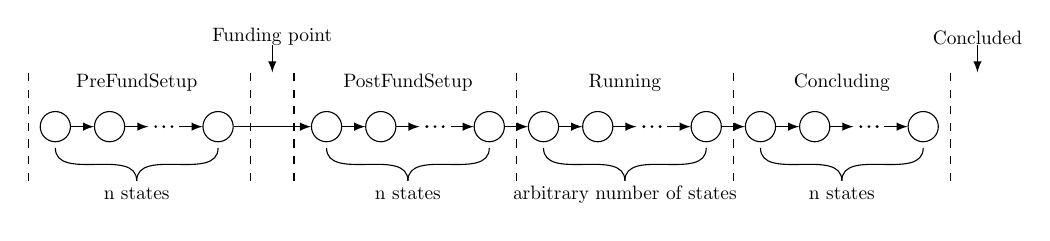
\begin{tikzpicture}[x=28pt,y=28pt,scale=0.7, every node/.style={transform shape}]
  \newcommand{\paperdiagram}[3]{%
    \begin{scope}[shift={(#1,0)}]
      % Circle
      \foreach \n in {0,1,3} {\node[circle,draw,text width=10pt,inner sep=0pt] (N\n#1) at (\n,0) {\strut};}
      % Transparent circle
      \foreach \n in {2} {\node[circle,draw,text width=10pt,inner sep=0pt,white] (N\n#1) at (\n,0) {\strut};}
      % Dots
      \foreach \n in {1.85,2,2.15} {\fill (\n,0) circle (0.8pt);}
      % Arrows
      \foreach \x [remember=\x as \lastx (initially 0)] in {1,2,3}{\draw[-latex] (N\lastx#1) -- (N\x#1);}
      % Under brackets with label #3
      \foreach \n in {0,3} {\draw ([shift={(0,-3pt)}]N\n#1.south) to[out=270,in=90] (1.5,-1) node[inner sep=1pt] (P) {\strut};}
      \node at (P.south) {\strut#3};
      % Upper label #2
      \node at (1.5,0.8) {\strut#2};
    \end{scope}
  }
  % Diagram nodes
  \paperdiagram{0}{PreFundSetup}{n states}
  \paperdiagram{5}{PostFundSetup}{n states}
  \paperdiagram{9}{Running}{arbitrary number of states}
  \paperdiagram{13}{Concluding}{n states}
  % Arrows between single diagram node
  \foreach \x [remember=\x as \lastx (initially 0)] in {5,9,13}{\draw[-latex] (N3\lastx) -- (N0\x);}
  % Vertical dashed
  \foreach \n in {-0.5,3.6,4.4,8.5,12.5,16.5} {\draw[dashed] (\n,-1) --++(90:2);}
  % Funding arrow
  \draw[latex-] (4,1) --++(90:0.5) node[at end,above,inner sep=0pt] {Funding point};
  \draw[latex-] (17,1) --++(90:0.5) node[at end,above,inner sep=0pt] {Concluded};
\end{tikzpicture}
}
  \caption{Cool, huh?}
\end{figure}
In the special case where the outcome of a channel is finalizable by all its participants, we say that the outcome is \textbf{universally finalizable}.
For a ForceMove channel, this happens at the following points in its lifecycle:
\begin{enumerate}
  \item After the first $n$ states have been broadcast. In this state, we say the channel is at the \textbf{funding point}.
  \item When a single conclusion proof is known to each participant. In this state, we say the channel is in the \textbf{concluded state}.
\end{enumerate}
It is an important property of ForceMove that all channels have one universally finalizable
state at the beginning of their lifecycle and one at the end
\footnote{If a channel does not end with a conclusion proof, it ends with an expired on-chain challenge,
in which case the outcome is already finalized on-chain.}.

If a participant has no finalizable outcomes, their analysis of the network needs to be performed
in terms of their \textbf{enabled outcomes}.
The enabled outcomes for a participant, $p$, is defined as the set of outcomes that $p$ has
no strategy to prevent from being finalized.
We write the set of enabled outcomes for $p$ as $\finalizable{\rchi}{\Omega_1 \dots \Omega_m}{(p)}$.

For any participant, $p$, in a channel, $\rchi$, exactly one of the following statements is
true at a given point in time:
\begin{enumerate}
  \item $p$ has at least one finalizable outcome.
  \item $p$ has at least two enabled outcomes.
\end{enumerate}
Note that if a participant has only enabled a single outcome, that outcome must be finalizable for them.

\subsection{Consensus Game}

Another important example of universally finalizable states comes from the \textbf{consensus game}.
The consensus game is a ForceMove \textit{application}, which means it specifies a certain
set of transitions rules that can be used to define the allowed state transitions for a ForceMove channel.
We will make heavy use of the consensus game throughout the paper.

The consensus game provides a way for participants to move from one universally finalizable outcome to another, provided that they all agree.
One participant proposes the new outcome, $\Omega_2$.
On their turn, each subsequent participant decides whether to accept the transition to the new outcome or whether to cancel the transition and return to the old outcome, $\Omega_2$.
\begin{figure}[h]\centering
  \makebox[\textwidth][c]{\begin{tikzpicture}[x=1.7cm, y=1cm]
  \begin{scope}[every node/.style={draw,circle,minimum size=4mm}]
    \node (A) at (0,0) {};
    \node (AB1) at (1,0) {};
    \node (AB2) at (2,0) {};
    \node[draw=none] (ABx) at (3,0) {};
    % Dots
    \foreach \n in {2.95,3,3.05} {\fill (\n,0) circle (0.8pt);}
    \node (ABn) at (4,0) {};
    \node (B) at (5,0) {};
  \end{scope}
  \begin{scope}
    \node at ([yshift=-0.5cm]A) { $A$ };
    \node at ([yshift=-0.5cm]AB1) { $(A, B, 1)$ };
    \node at ([yshift=-0.5cm]AB2) { $(A, B, 2)$ };
    \node at ([yshift=-0.5cm]ABn) { $(A, B, n-1)$ };
    \node at ([yshift=-0.5cm]B) { $B$ };
  \end{scope}
  \begin{scope}[-{Latex[length=2mm]}]
    \draw (A) to (AB1);
    \draw (AB1) to (AB2);
    \draw (AB2) to (ABx);
    \draw (ABx) to (ABn);
    \draw (ABn) to (B);
    \draw (AB1) to[bend right] (A);
    \draw (AB2) to[bend right] (A);
    \draw (ABn) to[bend right] (A);
  \end{scope}
\end{tikzpicture}
}
  \caption{
    A consensus game transition from $\Omega_1$ to $\Omega_2$, for a channel with $n$ participants.
    The counter records how many participants have approved the transition.
    If all participants agree, they finish in a state with outcome $\Omega_2$.
    Any participant can reject the transition, returning to the state with $\Omega_1$.
  }
\end{figure}

Throughout the only enabled outcomes for any participant are $\Omega_1$ and $\Omega_2$.
In particular, a participant has the finalizable outcome $\finalizable{\rchi}{\Omega_1}{p}$ until they approve the transition, and then enabled outcomes $\finalizable{\rchi}{\Omega_1, \Omega_2}{(p)}$ until they receive the final state.
When the final state is broadcast, every participant has the finalizable outcome $\finalizable{\rchi}{\Omega_2}{p}$.

\subsection{Outcomes First}

In practice, it is hard to write networks states down concisely.
Instead, we will write our constructions in terms of outcomes and use the properties of the consensus game to reason that (a) network states exist that lead to this outcome and (b) we can find a sequence of network states to transition from one outcome to another.

In particular

- if I have two network outcomes that differ in the outcome of a single CG channel
- then I can find a sequence of single-update network states that interpolate between them

- write down a sequence of outcomes
- update one channel at a time
- and have the same value to all participants

- the start and conclude states are also finalizable

\begin{figure}[h]\centering
  \makebox[\textwidth][c]{\begin{tikzpicture}[node distance=1cm]
  \node (s0) {
    \begin{tikzpicture}[x=0.7cm]
      \node[circAB, label=right:$L$] (L) at (0, 0) {};
      \node[circA, label=below:$A$] (A) at (-1, -1) {};
      \node[circB, label=below:$B$] (B) at (1, -1) {};
      \draw[->] (L) edge node[midway, left] { $3$ } (A);
      \draw[->] (L) edge node[midway, right] { $4$ } (B);
    \end{tikzpicture}
  };
  \node[right=of s0.south east, anchor=south west] (s1) {
    \begin{tikzpicture}[y=1cm, x=0.7cm]
      \node[sqadj] (a0) at (1, 0) {};
      \node[circAB, label=right:$L$] (p0) at (1, -1) {};
      \node[circA, label=below:$A$] (p1) at (0, -2) {};
      \node[circB, label=below:$B$] (p2) at (2, -2) {};

      \draw[->] (a0) edge node[midway, left] { $7$ } (p0);
      \draw[->] (p0) edge node[midway, left] { $3$ } (p1);
      \draw[->] (p0) edge node[midway, right] { $4$ } (p2);

    \end{tikzpicture}
  };

  \node[right=of s1.north east, anchor = north west] (s2) {
    \begin{tikzpicture}[y=1cm, x=2cm]
      \node[sqadj] (a0) at (1, 0) {};
      \node[circAB, label=right:$L$] (p0) at (1, -1) {};

      \draw[->] (a0) edge node[midway, left] { $7$ } (p0);

    \end{tikzpicture}
  };

  \node[right=of s2.north east, anchor=north west] (s3) {
    \begin{tikzpicture}[y=1cm, x=2cm]
      \node[sqadj] (a0) at (1, 0) {};
      \node[circAB, label=right:$L$] (p0) at (1, -1) {};
      \node[circA, label=below:$A$] (p1) at (0.58, -2) {};
      \node[circB, label=below:$B$] (p2) at (1.42, -2) {};

      \draw[->] (a0) edge node[midway, left] { $7$ } (p0);
      \draw[->] (p0) edge node[midway, left] { $6$ } (p1);
      \draw[->] (p0) edge node[midway, right] { $1$ } (p2);

    \end{tikzpicture}
  };

  \node[right=of s3.north east, anchor=north west] (s4) {
    \begin{tikzpicture}[y=1cm, x=1cm]
      \node[sqadj] (a0) at (1, 0) {};
      \node[circA, label=below:$A$] (p0) at (1, -1) {};
      \node[sqadj] (a1) at (2, 0) {};
      \node[circB, label=below:$B$] (p1) at (2, -1) {};

      \draw[->] (a0) edge node[midway, left] { $6$ } (p0);
      \draw[->] (a1) edge node[midway, left] { $1$ } (p1);

    \end{tikzpicture}
  };
  \node (mid) at ([yshift=-3mm] s0.north) {};
  \begin{scope}[-{Latex[length=2mm]}]
    \draw (s0.east |- mid) to (s1.west |- mid);
    \draw (s1.east |- mid) to (s2.west |- mid);
    \draw (s2.east |- mid) to (s3.west |- mid);
    \draw (s3.east |- mid) to (s4.west |- mid);
  \end{scope}

  \node[below=-1mm of s0] (below) { (a) };
  \node at (s1 |- below) { (b) };
  \node at (s2 |- below) { (c) };
  \node at (s3 |- below) { (d) };
  \node at (s4 |- below) { (e) };
\end{tikzpicture}
}
  \caption{
    In (a), $A$ and $B$ have exchanged the first two states in the channel $L$, bringing them to the funding point. At this point the channel is not yet funded.
    In step (b), both participants have deposited into the adjudicator.
    In step (c), the channel $L$ is running.
    $A$ and $B$ do not have a finalizable outcome and the ultimate outcome is governed by the rules given by the channel's game library.
    In step (d), $A$ and $B$ have created a conclusion proof and therefore have another universally finalizable outcome.
    They are then able to finalize this outcome on-chain and withdraw their funds in (e).
  }
\end{figure}
